
\documentclass[xcolor={dvipsnames}]{beamer}
\usepackage{amsmath}
% \usepackage{beamerthemesplit} // Activate for custom appearance
\usepackage{hyperref}
\usepackage{ragged2e}
\usepackage{amssymb}
\usepackage{verbatim}
\usepackage{lmodern}
\usepackage{url}
\usepackage{courier}


\title{Gradient Descent and such}
\author{Schwartz}
\date{\today}



\begin{document}

\frame{\titlepage}

\frame
{
 \frametitle{A brief history of Optimization}

\vspace{-.3cm}

\tiny
\begin{columns}
\begin{column}{.5\textwidth}

\vspace{-.1cm}

\begin{itemize}
\item[300 bc] Euclid considers minimal distance from point to a line
\& proves square is the greatest area rectangle 

\item[1615] Kepler optimizes dimensions of wine barrel \& formulates an early version of the (classical) secretary problem while looking for a new wife

\item[1636] Fermat shows derivatives vanish at extremes \& light travels between two points in minimal time

\item[1660s] Newton \& Leibniz create the mathematical basis of calculus 
and hence optimization calculus

\item[1696]  Johann \& Jacob Bernoulli study Brachistochrone problem -- calculus optimization is born

\item[1712] K\"{o}nig shows that the shape of honeycomb is optimal. The French Academy of Sciences declares the phenomenon as divine guidance

\item[1740] Euler's publication begins the research on a general theory of calculus optimization

\item[1754] Lagrange makes his first of many findings regarding calculus optimization at age 19 

\item[1900's] The first optimization algorithms are presented by Weierstrass, Steiner, Hamilton and Jacobi

\item[1806] Legendre presents the least square method, which also Gauss claims to have invented

\item[1815] ``The Law of Diminishing Returns" (introduced simultaneously by Malthus, Torrens, West, and Ricardo) uses a (quasi) concave function

\item[1826] Fourier formulates linear programming (LP) for solving mechanics and probability problems

\item[1847] Cauchy presents the gradient method

\end{itemize}

\end{column}
\begin{column}{.53\textwidth}

\begin{itemize}
\item[1857] Gibbs shows chemical equilibrium is minimum energy 

\item[1870s] The marginalist revolution in economics shifts the focus of economists to maximizing individuals utility 

\item[1880s] Convexity theory created -- Jensen introduces convex functions in 1905 -- 
 Minkowski convex sets in 1911
 
% , the idea has already appeared in the works of Hadamard (1883), H\"{o}lder (1889), and Stolz (1893).  , the earliest study on convex geometry was published by Brunn in 1887

\item[1917] Hancock publishes the first text book on optimization: ``Theory of Minima and Maxima''

\item [1917]Thompson's ``On Growth and Form'' applies optimization to analyze the forms of living organisms

\item[1928] Ramsey studies optimal economic growth which becomes optimal growth theory in the 1950's

\item[1932] Menger generalizes the traveling salesman problem

\item[1939] Kantorovich presents LP-model \& solution algorithm 
and receives Nobel prize in 1975 with Koopmans 

\item[1944] Neuman and Morgenstern, and Wald (1947) solve 
sequential problems w/ dynamic programming (DP)

\item [1947] Dantzig (USAF) presents the Simplex method for LP-problems, Neumann establishes duality theory

\item[1950's] Electronic calculation initiates algorithmic research

\item[1951] Markowitz presents portfolio theory using quadratic programing (QP) 
and receives the 1990 Nobel prize

\item[1954] Ford \& Fulkerson introduce combinatorial optimization for network research problems

\item[1960's] Space race sparks optimal control theory research

\item[1970s] Complexity analysis influences optimization theory
\item[1980's] Heuristic global optimization algorithms for large scale problems gain popularity
as computers improve
\end{itemize}

\end{column}
\end{columns}


}



\frame
{
\LARGE
 \frametitle{Objectives}

\begin{itemize}
\item Loss Function
\item Cost Function 
\item Objective Function
\item[]
\item Gradient Descent
\item Stochastic Gradient Descent
\item Newton's Method
\end{itemize}

\begin{figure}
\centering

%which Optimize Cost Functions\\${}$\\
\normalsize
%we gon' t'wirk alot on logistic regression...
 
\end{figure}

}

\frame
{
\normalsize
\frametitle{Exercise of the day}

\huge
\vspace{-2em}
$$\text{Find parameters that maximizes}$$
\vspace{-2em}
$$\text{the fit of model to data}$$
\vspace{-1em}
\onslide<2->{$$\iff$$
\vspace{-1em}
$$\text{minimize distance between}$$ 
\vspace{-2em}
$$\text{predicted and observed values}$$}
\vspace{-1em}
\onslide<3->{$$\iff$$
\vspace{-1em}
$$\hat Y_i \approx Y_i$$}
}

\frame
{
\frametitle{Regression Loss Functions}
\vspace{-2.5em}
\Huge
\only<4>{\vspace{-.2em}}
$$\only<5>{L_\delta(}\only<4>{ln(cosh(}\only<3>{|}\only<2>{\hspace{.4em}(}Y_i - \hat Y_i\only<2>{)^2}\only<3>{|}\only<4>{))\hspace{2.6em}}\only<5>{)\hspace{1em}}$$

\normalsize
\only<4>{\hspace{1.5in}\textcolor{green}{the good ol' \emph{hyperbolic cosine} function}
\vspace{-1.45em}
}


\textcolor{white}{\only<-4>{$$L_\delta(a) = \left\{ \begin{array}{ll}\frac{1}{2}a^2&: |a| < \delta \\\delta(|a|-\frac{1}{2}\delta) &: o.w.\end{array}\right.$$}}
\only<5>{$$L_\delta(a) = \left\{ \begin{array}{ll}\frac{1}{2}a^2&: |a| < \delta \\\delta(|a|-\frac{1}{2}\delta) &: o.w.\end{array}\right.$$}

\only<4>{\vspace{-.09em}}
\only<5>{\vspace{.125em}}
\vspace{-.5em}
\begin{figure}
\centering
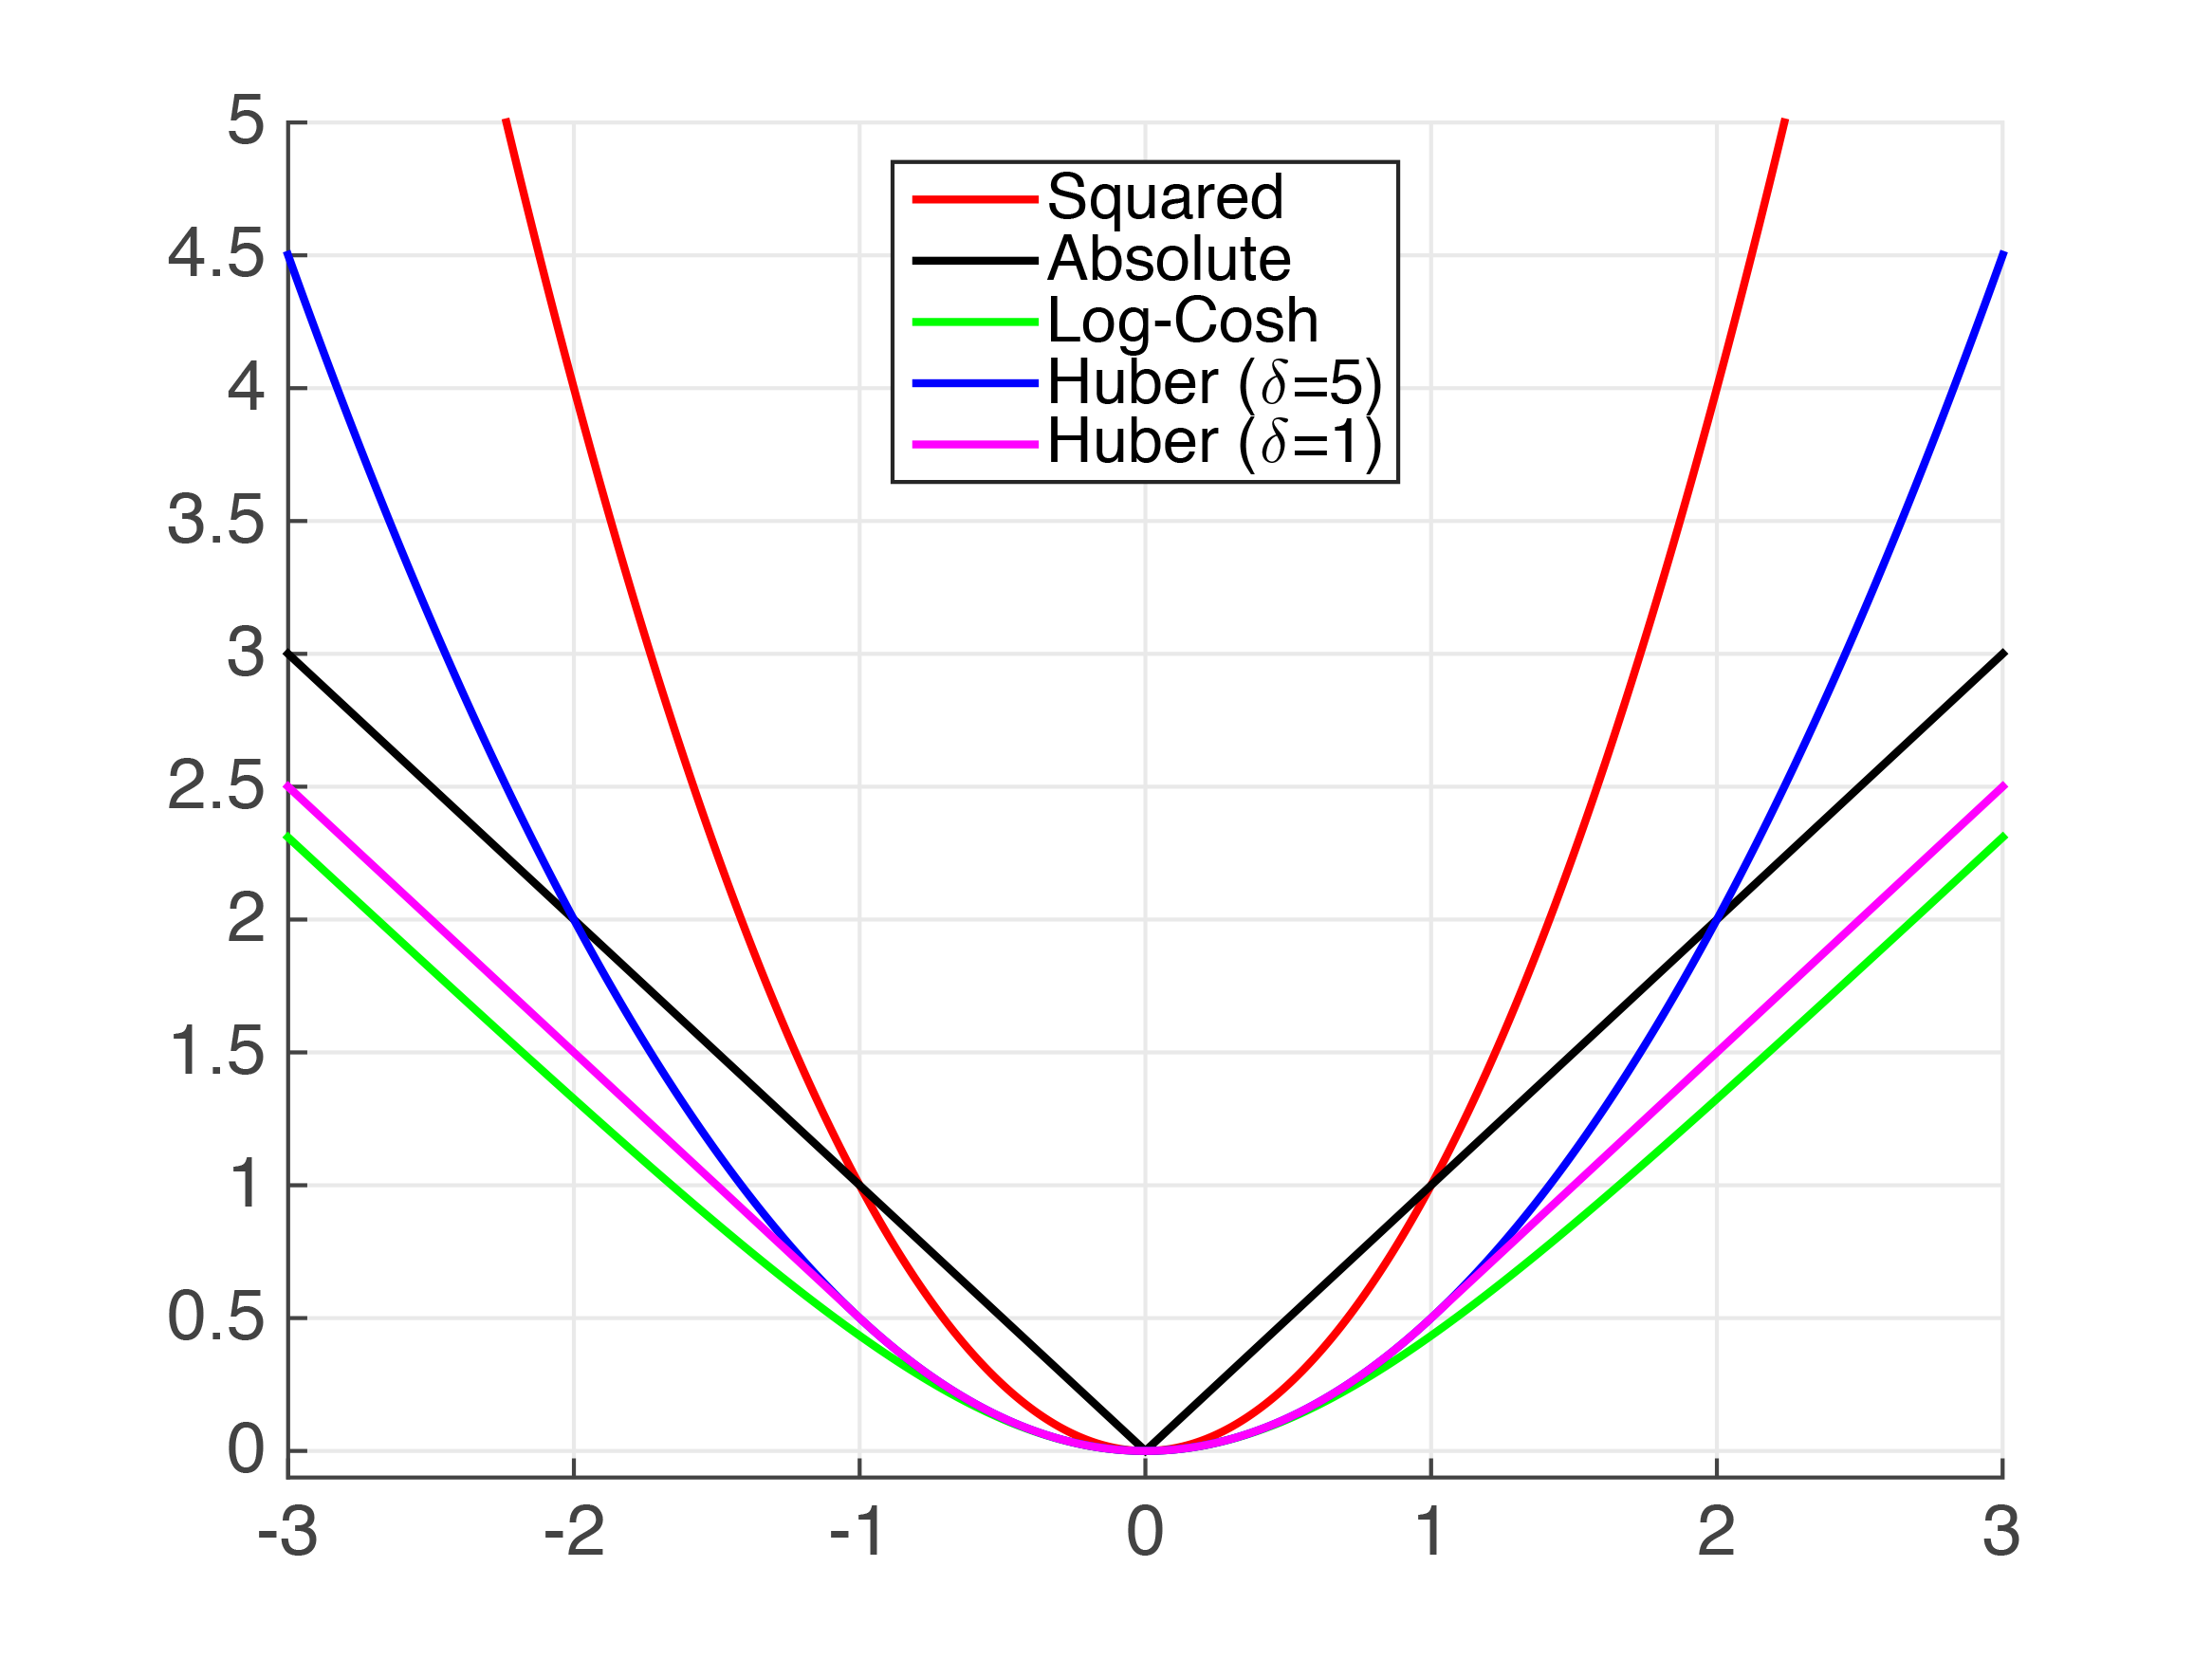
\includegraphics[width=3in]{regressionlosses.png}
\end{figure}

}

\frame
{
\frametitle{Classification Loss Functions}

\vspace{-.85in}

$$\textcolor{red}{Y \in \{0,1\}}: \underset{p}{min}-Y \log p - (1 - Y) \log (1-p) \quad\quad p = \frac{1}{1+e^{-x^T\boldsymbol\beta}}$$
\onslide<2->{$\iff$
$$\textcolor{red}{Y \in \{-1,1\}}: \underset{p}{min} \frac{1}{ln 2} ln \left(1 + e^{-Y ln\left(\frac{p}{1-p}\right)}\right) \quad\quad\quad  ln\left(\frac{p}{1-p}\right) = x^T\boldsymbol\beta$$}

\vspace{-.25in}

\begin{figure}
\centering
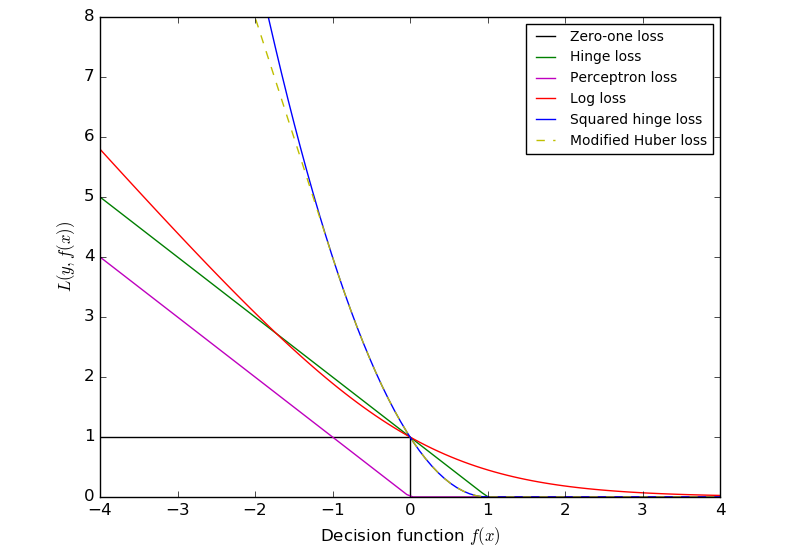
\includegraphics[width=3in]{loss.png} 
\end{figure}

\small
\vspace{-1.5in}
\hspace{2in}$Y=1$ Loss Functions

\hspace{2in}\textcolor{gray}{$Y=0$ is mirror image}


}


\frame
{
\normalsize
\frametitle{Cost function}

\begin{itemize}
\item<1> $\sum (Y_i - x_i^T\beta)^2$ 
\vspace{-1.5em}
\item<2-> $\sum (Y_i - x_i^T\beta)^2 = ({\boldsymbol Y} - {\boldsymbol x}{\boldsymbol\beta})^T({\boldsymbol Y} - {\boldsymbol x}{\boldsymbol\beta}) \textcolor{red}{\;= ||{\boldsymbol Y} - {\boldsymbol x}{\boldsymbol\beta}||^2}$ \onslide<5->{\textcolor{blue}{$+ \lambda ||\beta||$}}
\item<3->[] This cost function is minimized at $\left({\boldsymbol x}^T{\boldsymbol x} \right)^{-1} {\boldsymbol x}^T {\boldsymbol Y}$
\item[]
\item[]
\item $-\sum Y_i \log g^{-1}(x_i^T{\boldsymbol \beta}) + (1 - Y_i) \log \left(1-g^{-1}(x_i^T {\boldsymbol \beta})\right)$ \onslide<5->{\textcolor{blue}{$+ \lambda ||\beta||$}}\\
$$g^{-1}(z) = \frac{1}{1+e^{-z}} $$
\item<4->[] This cost function is minimized at... \footnotesize oh, no analytical solution... \normalsize
\item[]<5->\textcolor{blue}{$\text{Regularized cost functions also don't have closed form solutions}$}
\end{itemize}
}


\frame
{
\normalsize
\frametitle{Objective function}

\begin{itemize}
\item An objective function is \underline{a target of an optimization procedure}
\item A cost function \emph{IS} an objective function \textcolor{gray}{(which we minimize)}
\item[]
\item<2-> But there are obviously \emph{other} objective functions
\item<2-> E.g., a likelihood is an objective function \textcolor{gray}{(which we maximize)}
\item<3-> \textcolor{Maroon}{MLE maximizes the (log) likelihood, e.g.,
$$\underset{{\boldsymbol\beta}}{argmax}\; (2\pi \sigma^2)^{-\frac{n}{2}} e^{-\frac{1}{2\sigma^2}(\textbf{Y} - \textbf{x}{\boldsymbol\beta})^T(\textbf{Y} - \textbf{x}{\boldsymbol\beta})}$$
or
$$\underset{{\boldsymbol\beta}}{argmax}\; \prod \left(\frac{1}{1+e^{-\textbf{x}_i^T\boldsymbol\beta }}\right)^{Y_i} \left(\frac{1}{1+e^{\textbf{x}_i^T\boldsymbol\beta}}\right)^{1-Y_i}$$}
\item<4-> But in Machine Learning \\
the standard orientation and nomenclature
is ``minimize cost"
\end{itemize}

}

\frame
{
\normalsize
\frametitle{Exercise of the day}

\huge
\vspace{-2em}
$$\text{Find parameters that maximizes}$$
\vspace{-2em}
$$\text{the fit of model to data}$$
\vspace{-1em}
\onslide<2->{$$\iff$$
\vspace{-1em}
$$\text{minimize distance between}$$ 
\vspace{-2em}
$$\text{predicted and observed values}$$}
\vspace{-1em}
\onslide<3->{$$\iff$$
\vspace{-1em}
$$\hat Y_i \approx Y_i$$}
}


\frame
{
\frametitle{Gradients}

For some function $f({\boldsymbol x})$, the gradient

$$\nabla_{\boldsymbol x} f\left({\boldsymbol x^{(0)}}\right) = \left(\frac{\partial f}{\partial x_1}\left({\boldsymbol x^{(0)}}\right), \frac{\partial f}{\partial x_2}\left({\boldsymbol x^{(0)}}\right), \cdots, \frac{\partial f}{\partial x_p}\left({\boldsymbol x^{(0)}}\right) \right)$$

\textcolor{gray}{collects the instantaneous slopes (derivatives) with respect to\\
each variable $x_j$ of ${\boldsymbol x}$ and then evaluates each one at point ${\boldsymbol x^{(0)}}$}\\${}$\\


\onslide<2->{\hspace*{-1.25em}\textcolor{red}{$\Rightarrow$} $\nabla f({\boldsymbol x^{(0)}})$ points in the direction of greatest \underline{increase} in $f$ at ${\boldsymbol x^{(0)}}$\\}

\vspace{.5em}

\onslide<3->{\hspace*{-1.25em}\textcolor{red}{$\Rightarrow$} The magnitude $|\nabla f({\boldsymbol x^{(0)}})|$ is proportional to $f$'s steepness at ${\boldsymbol x^{(0)}}$}

\begin{figure}
\centering
\onslide<4->{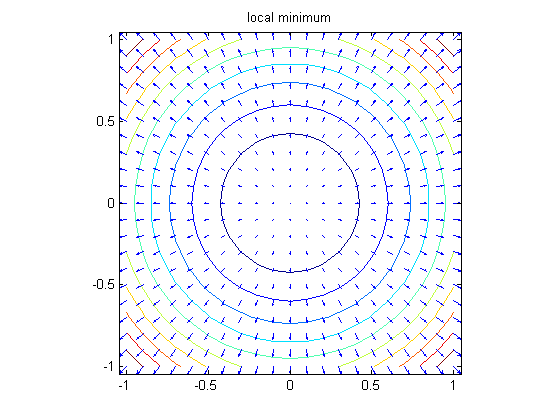
\includegraphics[width=2in]{gradients_02.png} 
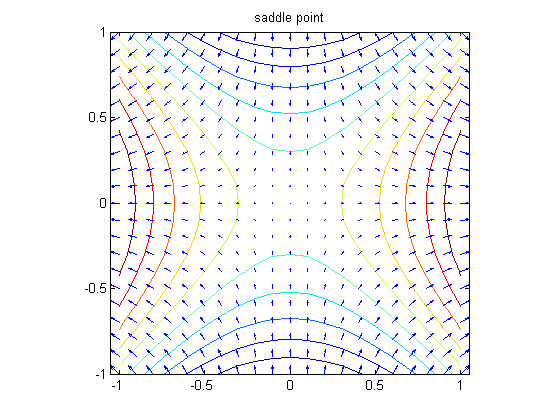
\includegraphics[width=2in]{gradients_04.png}}
\end{figure}

}


\frame
{
\frametitle{Gradient Descent}

\footnotesize
\begin{figure}
\centering
\url{http://vis.supstat.com/2013/03/gradient-descent-algorithm-with-r/}
\end{figure}
\normalsize

\begin{enumerate}
\item[0.] Choose step size $\alpha$ and precision threshold $\epsilon$
\item Select starting point ${\boldsymbol x^{(0)}}$, set $i = 1$
\item Update ${\boldsymbol x^{(t)} = {\boldsymbol x}^{(t-1)}} - \alpha \nabla f({\boldsymbol x^{(t-1)}})$
\item If $\frac{|f({\boldsymbol x}^{(t-1)})| - |f({\boldsymbol x}^{(t)})|}{|f({\boldsymbol x}^{(t-1)})|} < \epsilon$, return \emph{min} $|f({\boldsymbol x}^{(t)})|$  \& \emph{argmin} ${\boldsymbol x}^{(t)}$ 
\item else, return to step 2. $ \quad\quad$ \onslide<2->{\textcolor{gray}{[how do we choose $\alpha$ and $\epsilon$?]}}
\item[]
\end{enumerate}


}




\frame
{
\frametitle{Step Size $\alpha$ and Stopping Criterion $\epsilon$}


\begin{itemize}
\item[]<1-> \textcolor{Maroon}{Here's one way to choose $\alpha$:}
\item<2-> If $\frac{|\nabla f({\boldsymbol a}) - \nabla f({\boldsymbol a'}) |}{|a - a'|} < c \in \mathbb{R}$,
choose $\alpha \leq 1/c$
\item<3-> E.g., if $f(x) = x^2$, then $\nabla f(x) = f'(x) = 2x$
\item<4-> So $\frac{|\nabla f({\boldsymbol a}) - \nabla f({\boldsymbol a'}) |}{|a - a'|} = \frac{2(a-a')}{(a-a')} = 2$, and $\alpha = 1/2$ is optimal
\item[]
\item<5->[]  \textcolor{Maroon}{And an (adaptive) way to choose $\alpha$} \only<8->{\footnotesize \textcolor{gray}{(relying on ``smoothness'' of $f$)}}\normalsize\textcolor{Maroon}{:} 
\item<6-> Let $\Delta {\boldsymbol x}^{(t)} = {\boldsymbol x}^{(t)} - {\boldsymbol x}^{(t-1)}$
\item[]<7-> and let $\Delta \nabla f({\boldsymbol x}^{(t)}) = \nabla f({\boldsymbol x}^{(t)}) - \nabla f({\boldsymbol x}^{(t-1)})$
\item<8-> For step $t+1$, let $\alpha = \frac{\Delta \nabla f({\boldsymbol x}^{(t)})^T \Delta {\boldsymbol x}^{(t)}}{||\Delta \nabla f({\boldsymbol x}^{(t)})||^2} \; \rightarrow \frac{\overset{\text{ \tiny \textcolor{gray}{large if the change in gradient is}}}{\text{ \tiny \textcolor{gray}{the same direction as just moved}}}}{\text{ \tiny \textcolor{gray}{large if the gradient is changing}}}$
\end{itemize}

\normalsize
\onslide<9->{\noindent\makebox[\linewidth]{\rule{\paperwidth}{0.4pt}}}

\begin{itemize}
\item[]<9->  \textcolor{Maroon}{And here's some potential stopping criterion:}
\begin{enumerate}
\item[a.]<10-> $\frac{|f({\boldsymbol x}^{(t-1)})| - |f({\boldsymbol x}^{(t)})|}{|f({\boldsymbol x}^{(t-1)})|} < \epsilon$
\item[b.]<11-> Max number of iterations
\item[c.]<12-> $|\nabla f| < \epsilon$
\end{enumerate}

\end{itemize}


}



\frame
{
\frametitle{Pitfalls (literally)}

\begin{figure}
\centering
\only<1-5>{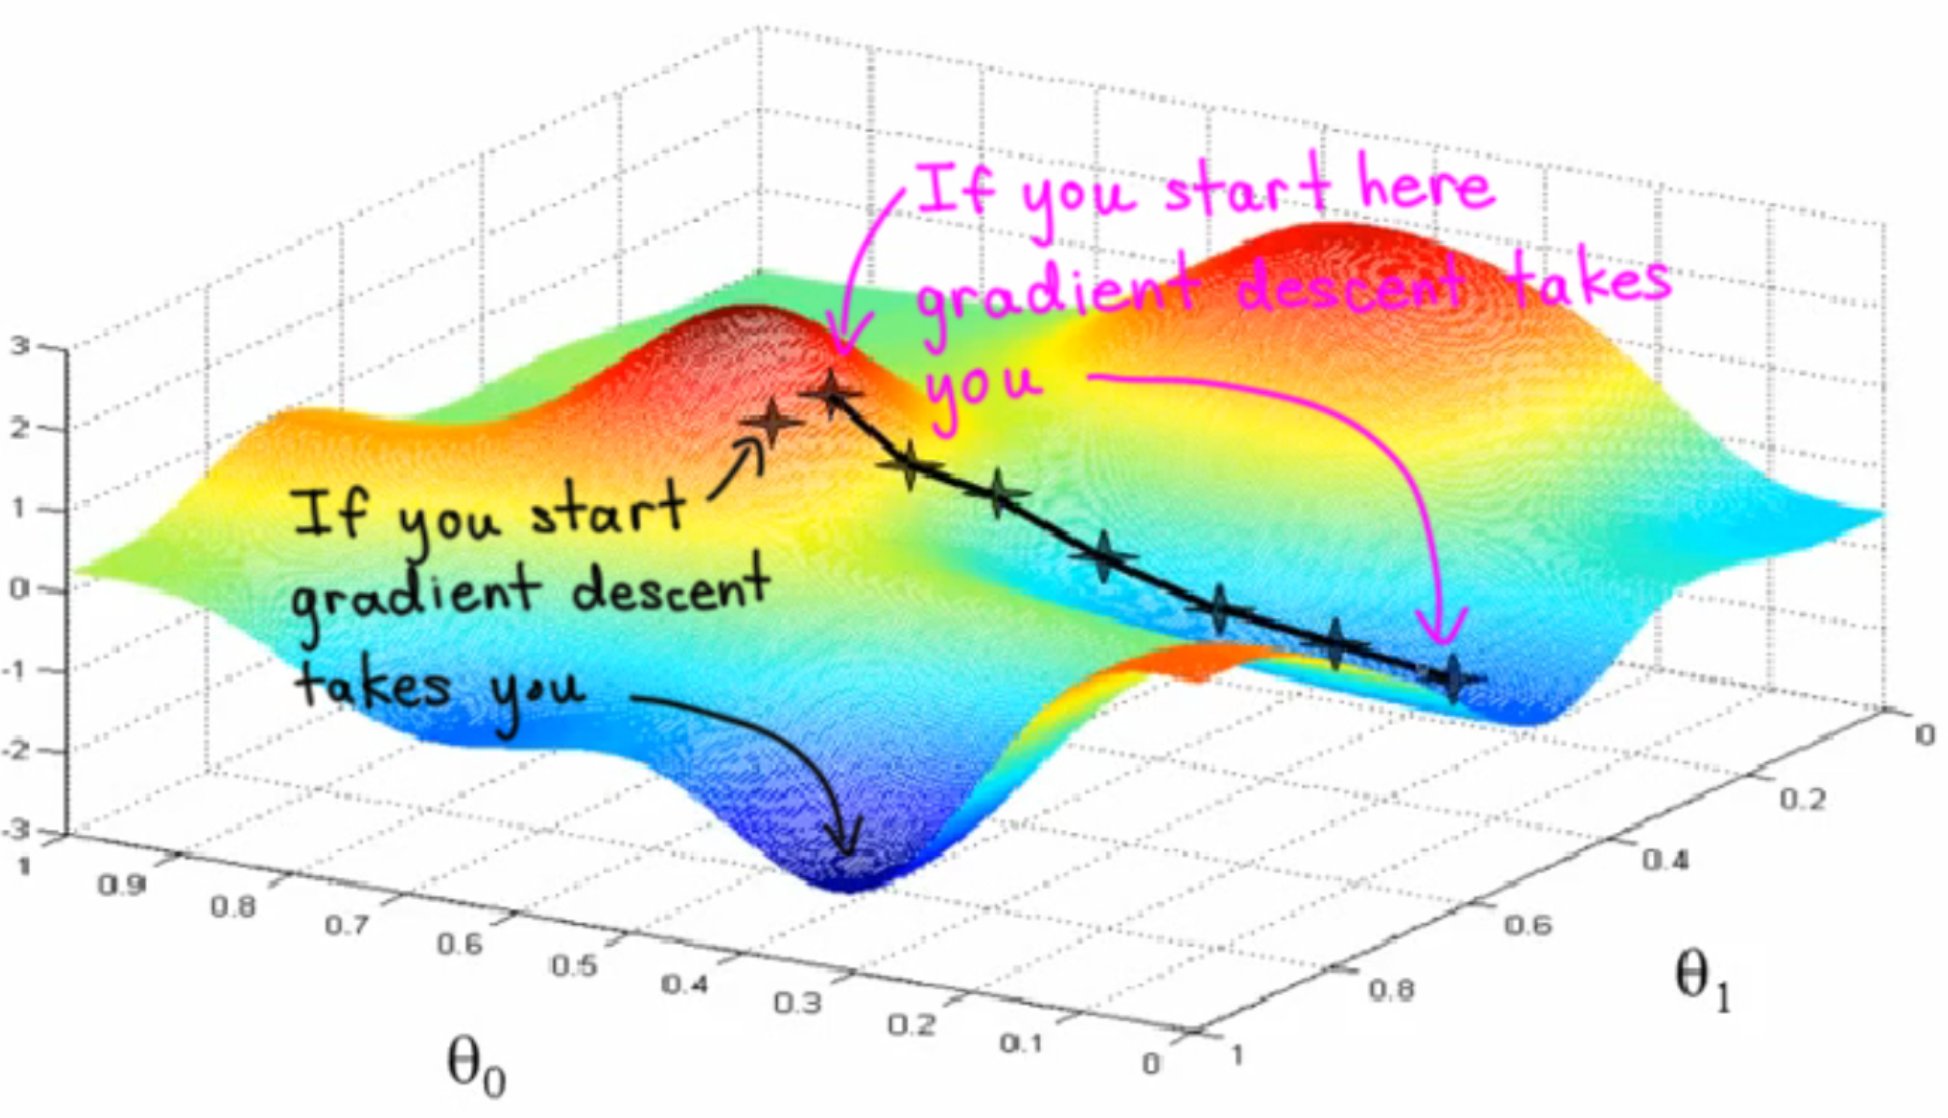
\includegraphics[height=2in]{localmaxima.png}} 
\only<6>{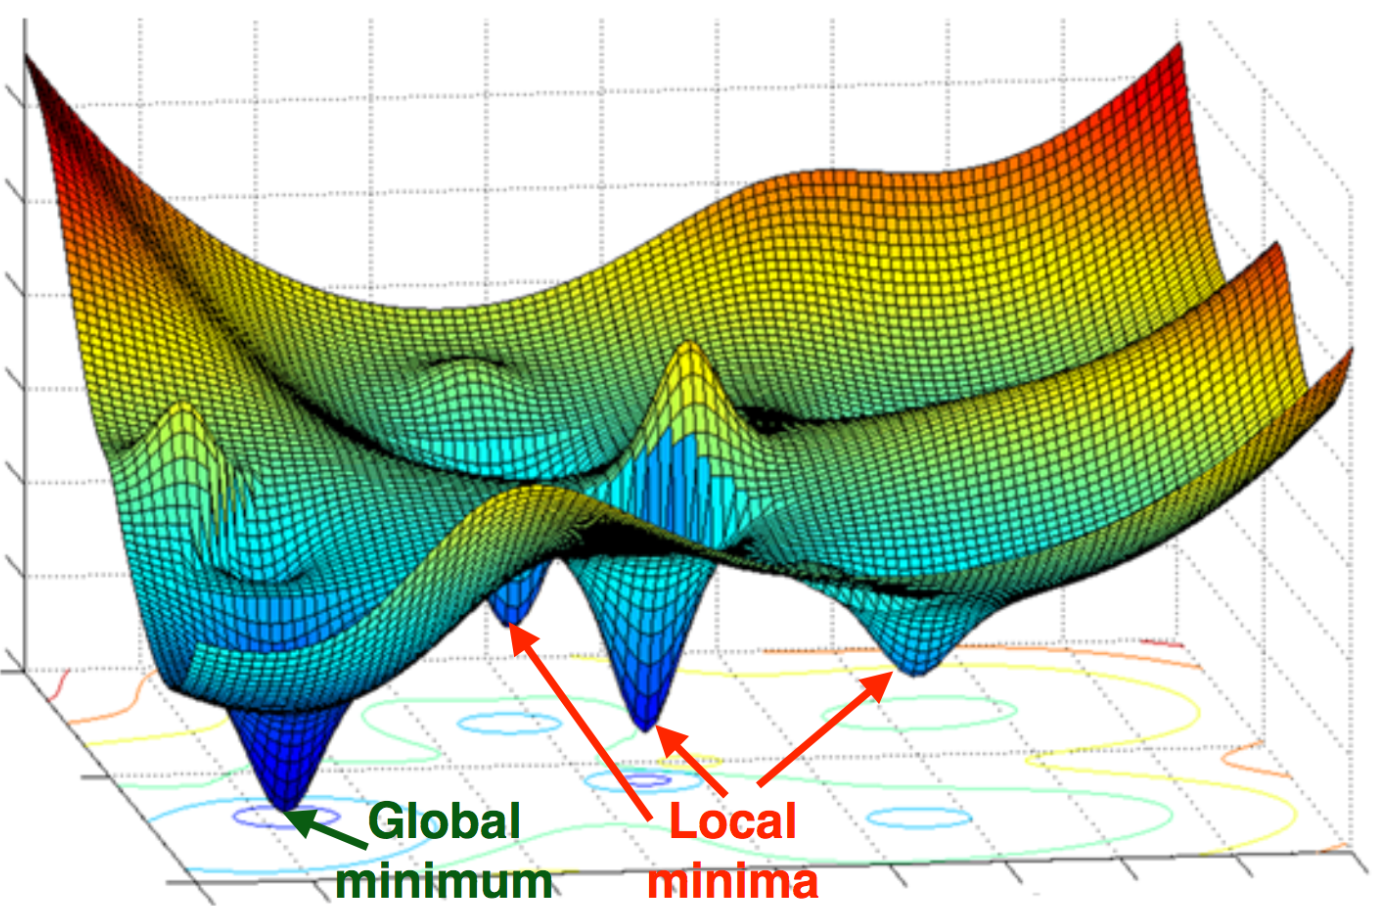
\includegraphics[height=2in]{minmax.png}}
\end{figure}

\vspace{-1em}

\begin{itemize}
\item<2-> \emph{Convexity} required to guarantee \emph{global minimum} 
\item<3-> \emph{Differentiable cost function} required for \emph{gradient descent}
\item<4-> Convergence is asymptotic...  
\item<5-> Good performance requires feature scaling \& parameter tuning 
\end{itemize}

}



\frame
{
\frametitle{Logistic regression}

% \lambda |\beta| derivative is \lambda
% \lambda ||\beta||^2/2 derivative is \lambda \beta


\vspace{-.25in}
$$L({\boldsymbol \beta}) = \sum Y_i \log g^{-1}(x_i^T{\boldsymbol \beta}) + (1 - Y_i) \log \left(1-g^{-1}(x_i^T {\boldsymbol \beta})\right) \onslide<13-14>{\textcolor{orange}{\;- \; \lambda \frac{1}{2}||\beta||^2}}
\hspace*{-1.85cm}\onslide<15-16>{\textcolor{orange}{\;- \; \lambda |\beta|}}
$$
$$\onslide<2->{\nabla L({\boldsymbol \beta}) = \;?}$$

\setlength{\leftmargini}{-40pt}
\begin{itemize}
\item[]<3-7>
\begin{align*}
\text{\textcolor{gray}{First}} \quad\quad\frac{d}{dz} g^{-1}(z) = {}&  \frac{d}{dz} \frac{1}{1+e^{-z}}\\
\onslide<4->{= {}&  \frac{d}{dz} (1+e^{-z})^{-1} }\\
\onslide<5->{= {}& -(1+e^{-z})^{-2}(-e^{-z})} \\
\onslide<6->{= {}& \frac{1}{1+e^{-z}} \frac{e^{-z}}{1+e^{-z}}}\\
\onslide<7->{= {}& g^{-1}(z) \left(1 - g^{-1}(z) \right)}
\end{align*}
\end{itemize}
\vspace{-2.5in}

\setlength{\leftmargini}{-17.5pt}
\begin{itemize}
\item[]<8-> 
\begin{align*}
{} &\frac{\partial}{\partial \beta_{\textcolor{red}{j}}}L({\boldsymbol \beta})
\quad\quad\quad\quad\quad\quad\quad\quad\quad\quad\quad\quad\quad\quad\quad\quad\quad\quad\quad\quad\quad\quad\quad \only<14>{\textcolor{orange}{- \lambda \beta }}\only<16>{\textcolor{orange}{\;\; \pm  \lambda }}
 \\
={}& \frac{\partial}{\partial \beta_j}
\left( \sum Y_i \log g^{-1}(x_i^T{\boldsymbol \beta}) + (1 - Y_i) \log \left(1-g^{-1}(x_i^T {\boldsymbol \beta})\right) \right) \\
\onslide<9->{={}& \sum \frac{\partial}{\partial \beta_j} g^{-1}(x_i^T{\boldsymbol \beta})
\left(\frac{Y_i}{g^{-1}(x_i^T{\boldsymbol \beta})} - \frac{(1 - Y_i)}{\left(1-g^{-1}(x_i^T {\boldsymbol \beta})\right)}\right)} \\
\onslide<10->{={}&\sum g^{-1}(x_i^T{\boldsymbol \beta}) \left(1 - g^{-1}(x_i^T{\boldsymbol \beta}) \right) \textcolor{red}{x_{ij}}
\left(\frac{Y_i}{g^{-1}(x_i^T{\boldsymbol \beta})} - \frac{(1 - Y_i)}{\left(1-g^{-1}(x_i^T {\boldsymbol \beta})\right)}\right)} \\
\onslide<11->{={}&\sum x_{ij} \left(Y_i\left(1 - g^{-1}(x_i^T{\boldsymbol \beta}) \right) - (1 - Y_i)g^{-1}(x_i^T{\boldsymbol \beta})  \right)} \\
\onslide<12->{={}&\sum x_{ij} \left(Y_i - g^{-1}(x_i^T{\boldsymbol \beta})  \right) = 
\textcolor{red}{\sum_{i=1}^n x_{ij} \left(Y_i -  \frac{1}{1+e^{-x_i^T{\boldsymbol \beta}}}  \right) = \sum_{i=1}^n x_{ij} (Y_i - \hat Y_i) } }
\end{align*}
\end{itemize}
}



\frame
{
\frametitle{Logistic regression}



$$\only<2>{\texttt{C}}\only<1>{\texttt{L}}({\boldsymbol \beta}) \;\;\; = \onslide<2>{-}\sum Y_i \log g^{-1}(x_i^T{\boldsymbol \beta}) + (1 - Y_i) \log \left(1-g^{-1}(x_i^T {\boldsymbol \beta})\right)$$

$$\only<2>{\nabla \texttt{C}}\only<1>{\nabla \texttt{L}}({\boldsymbol \beta}) \;\;\; = \onslide<2>{-}\left[ \begin{array}{c}
\sum x_{i1} \left(Y_i -  \frac{1}{1+e^{-x_i^T{\boldsymbol \beta}}}  \right)\\
\sum x_{i2} \left(Y_i -  \frac{1}{1+e^{-x_i^T{\boldsymbol \beta}}}  \right)\\
\vdots\\
\sum x_{ip} \left(Y_i -  \frac{1}{1+e^{-x_i^T{\boldsymbol \beta}}}  \right)
\end{array}\right]$$

${}$\\${}$\\

$${\boldsymbol \beta^{(t)} = {\boldsymbol \beta}^{(k-1)}} \only<1>{+}\only<2>{-} \alpha\only<2>{\nabla \texttt{C}}\only<1>{\nabla \texttt{L}}({\boldsymbol \beta^{(k-1)}})$$

}


\frame
{
\frametitle{Potential Gradient Descent Drawbacks}

\begin{enumerate}
\item<1-> Memory (data needs to fit)
\item<1-> Processor (cost function over all rows is expensive)
\end{enumerate}
}

\frame
{
\frametitle{Potential Gradient Descent Drawbacks \emph{Solutions}}

\begin{itemize}
\item \textcolor{Maroon}{Observations contribute equal weight to the gradient} 

$$\frac{\partial L_{1,\cdots n}}{\partial \beta_j} ({\boldsymbol \beta}) = 
\textcolor{red}{\sum_{i=1}^n} x_{ij} \left(Y_i -  \frac{1}{1+e^{-x_i^T{\boldsymbol \beta}}}  \right) $$

\item<2-> \textcolor{Maroon}{We could just use only a single data point at each iteration?} 
$$\frac{\partial L_i}{\partial \beta_j} ({\boldsymbol \beta}) = 
x_{ij} \left(Y_i -  \frac{1}{1+e^{-x_i^T{\boldsymbol \beta}}}  \right) $$

\item<3-> \textcolor{Maroon}{The expected direction of the gradient would stay the same}
$$ \frac{1}{n} \text{E}\left[\frac{\partial L_{1,\cdots n}}{\partial \beta_j} ({\boldsymbol \beta})\right] = \text{E}\left[\frac{\partial L_i}{\partial \beta_j} ({\boldsymbol \beta})\right] $$
\item<4-> \textcolor{Maroon}{We could also use a batch of data points at each iteration}
\item[]
\item[]<5-> \textcolor{NavyBlue}{This would address memory/processing limitations}
\item[]<6-> \textcolor{red}{\underline{It has been empirically proven to also often converge faster!}}
\item[]<7-> \textcolor{gray}{It does tend to oscillate around as it nears the minimum...}
\item[]
\end{itemize}
}

\frame
{
\frametitle{Newton-Raphson}

\begin{itemize}
\item[] \textcolor{Maroon}{Gradient Descent}
$${ x^{(t)} = { x}^{(t-1)}} - \alpha f'\left({ x^{(t-1)}}\right)$$

$${\boldsymbol x^{(t)} = {\boldsymbol x}^{(t-1)}} - \alpha \nabla f\left({\boldsymbol x^{(t-1)}}\right)$$


\item[]<2-> \textcolor{Maroon}{Newton-Raphson}
$${ x^{(t)} = { x}^{(t-1)}} - \frac{f'\left(x^{(t-1)}\right)}{f''\left(x^{(t-1)}\right)}$$

$${\boldsymbol x^{(t)} = {\boldsymbol x}^{(t-1)}} -  \left[\texttt{H}f\left({\boldsymbol x^{(t-1)}}\right)\right]^{-1} \nabla f\left({\boldsymbol x^{(t-1)}}\right)$$

\onslide<3->{$$ \texttt{H}f({\boldsymbol x}) = {\textbf{\texttt{H}}}, \text{ where } {\textbf{\texttt{H}}}_{ij} = \frac{\partial f}{\partial x_i \partial x_j}\left({\boldsymbol x^{(0)}}\right)$$}

\item<4-> 2nd order information makes Newton-Raphson faster
\item<5-> Inverting the Hessian matrix can be costly (or impossible)
\item<6-> Newton-Raphson can diverge with an initial bad guess 
\item[]

\end{itemize}
}


\frame
{
\frametitle{Conclusions}

\begin{itemize}
\item Best Method?
\item<2->[]Depends
\item<3-> Inventing New Cost functions? 
\item[]<4->Probably not
\item<5-> So why are we doing this? 
\item<6->[] Fitting models is just optimizing... knowing how it works could help you apply model fitting procedures more effectively 
\item<6->[]
\item<6->[]
\item<7->[]Bonus: \\ \footnotesize
\url{http://cs229.stanford.edu/notes/cs229-notes1.pdf}
\end{itemize}
}


\end{document}











